\chapter{Durchführung}

\section{Durchführung Versuch 25: Oszilloskop}

\subsection{Aufgabe 1: Bedienung des Oszilloskops}
Zunächst wird der Funktionsgenerator an \textbf{Kanal 1} des Oszilloskops angeschlossen. Als Signalfunktion wird ein \textbf{Sinus mit einer Frequenz von ca. 100\,Hz} gewählt. Über die Kanaltaste wird sichergestellt, dass für die Dämpfung der Wert \textbf{1X} eingestellt ist, da sonst die gemessenen Spannungen verzerrt dargestellt werden.

Nachdem der Trigger korrekt eingestellt wurde, sollte das Signal als \textbf{stehendes Bild} sichtbar sein. Anschließend werden die \textbf{Scale-Regler} für das Vertikal- und Horizontalfeld sowie die \textbf{Positionsregler} getestet, um die Auswirkungen auf das Oszilloskopbild zu beobachten. Die horizontale Position wird danach wieder symmetrisch eingestellt.

Im Triggerfeld wird der Modus auf \textbf{Auto} gesetzt. Mit Hilfe des \textbf{Level-Reglers} lässt sich beobachten, wie sich das Signal an der Triggerposition verschiebt. Liegt der Triggerlevel außerhalb des Signals, erfolgt keine Triggerung, das Signal wird aber weiterhin angezeigt. Danach wird der Modus auf \textbf{Normal} umgeschaltet, und die Auswirkungen der \textbf{Triggerflanke} werden untersucht. Alle Beobachtungen werden im Protokoll dokumentiert.

\subsection{Aufgabe 2: Amplituden- und Zeitmessung}

\subsubsection{Signale 1–4}
Der Signalgenerator erzeugt verschiedene Signale mit unterschiedlicher Amplitude und Frequenz. Über die Taster können die Signale ausgewählt werden. Der Ausgang 2 des Signalgenerators wird mit Kanal 1 des Oszilloskops verbunden, und die Versorgungsspannung wird eingeschaltet.

Die \textbf{Nulllage des Signals} wird eingestellt, indem die Kopplung auf \textbf{Erde} gesetzt und die Signalmitte in die vertikale Bildschirmmitte verschoben wird. Danach wird die Kopplung wieder auf \textbf{DC} gestellt.

Für jedes Signal werden folgende Größen gemessen:
\begin{itemize}
    \item Periodendauer / Frequenz
    \item Spitze-Spitze-Spannung (USS) und Gleichspannungsanteil
    \item Bild oder Skizze des Signals
\end{itemize}
Die Messungen erfolgen sowohl mit der \textbf{Cursor-Funktion} als auch mit den \textbf{automatischen Messfunktionen}, wobei der Fehler für die Cursor-Messung aus der Ablesegenauigkeit abgeschätzt wird. Die Signale werden auf einem USB-Stick gespeichert.

\subsubsection{Signal 5}
Signal 5 zeigt einen \textbf{periodisch exponentiell abfallenden und ansteigenden Verlauf} (Lade- und Entladevorgang eines Kondensators). Hier wird die \textbf{DC-Kopplung} eingestellt, da die AC-Kopplung zu Verzerrungen führt. Es wird die \textbf{Halbwertszeit} des Signals gemessen. Die Zeitbasis wird so gewählt, dass der größte mögliche Zeitbereich sichtbar ist.

\subsubsection{Signale 6–8 (qualitativ)}
\begin{itemize}
    \item \textbf{Signal 6:} Wellenpakete unterschiedlicher Höhe werden ausgesendet. Mit \textbf{Auto-Triggerung} erscheinen die Pakete nur kurz. Durch \textbf{manuelle Triggerung} können gezielt einzelne Pakete dargestellt werden.
    \item \textbf{Signal 7:} Beobachtung im Auto-Modus. Der Triggerlevel muss angepasst werden, um eine stabile Anzeige zu erhalten.
    \item \textbf{Signal 8:} Beide Kanäle des Oszilloskops werden aktiviert. Kanal 1 ist verrauscht, Kanal 2 sauber. Die Triggerung erfolgt auf Kanal 2, um beide Signale stabil darzustellen.
\end{itemize}

\subsubsection{Signal 9: Frequenzspektrum}
Signal 9 zeigt eine \textbf{Schwebung}, d.h. die Überlagerung zweier Sinussignale. Nach Aktivierung der \textbf{AC-Kopplung} und Stopp des Signals wird die \textbf{Schwingungsfrequenz $f_1$} und die \textbf{Schwebungsfrequenz $f_2$} mittels Cursor bestimmt. Anschließend wird die \textbf{Fouriertransformation (FFT)} genutzt, um die Grundfrequenzen $f_I$ und $f_{II}$ zu messen.

\subsection*{Ausführliche Ablesefehleranalyse}
In diesem Teil soll aufgeschlüsselt werden, wie hoch die Ablese Ungenauigkeit der Cursor-Funktion des Oszilloskops ist. 
Dazu betrachten wir zunächste den Aufbau des Displays. 

\begin{figure} [h!]
    \centering
        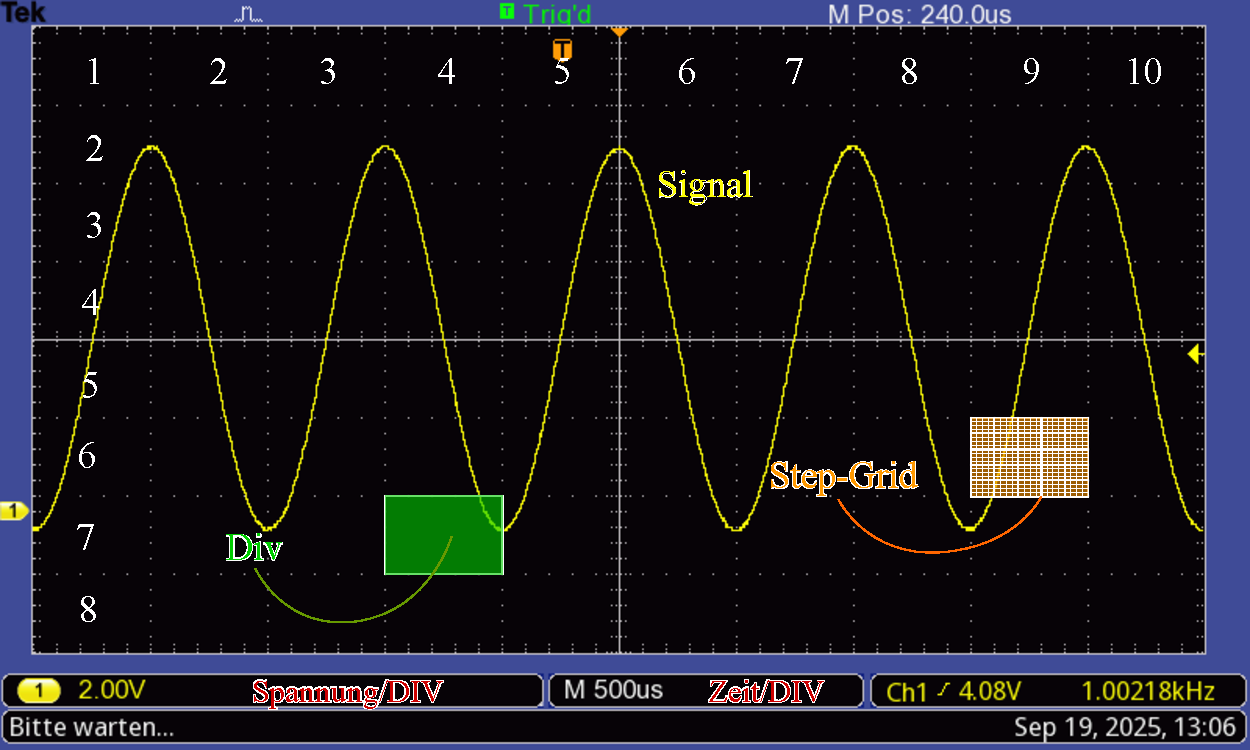
\includegraphics[width=0.45\textwidth]{img/25/SinusVis.pdf}
    \caption{Beispiel aus dem Versuch. 8 mal 10 DIVs.}
\end{figure}

Es werden dabei immer $8 \times 10$ DIVs angezeigt. Die $8$ sind die Amplituden in $[V]$ und die $10$ die Zeitachse $[s]$. Beide Achsen können dabei seperat in ihrer Größe verändert werden.
Insgesamt besteht jeder DIV aus $25 \times 25$ >>steps<<\footnote{Steps ist nicht der formale Begriff, sondern der von mir genutzte}. Jeder Setep ist dabei die Position, an der ein Cursor stehen kann. 
Für einen Gesamten DIV hat somit $200$ Steps auf der Vertikalen und $250$ Stept auf der Horizontalen. 

Darüber lässt isch nun immer der Mindestabstand bestimmen, den zwei Cursor messen können. 50\% dieses Abstandes (also der Zeit- bzw. Spannungsdifferenz) sind dann der Ablesefehler des Oszilloskops.
Damit haben wir einen immergleichen prozentualen Fehler der Cursorgenauigkeit. 

Spannungsungenauigkeit:
\begin{equation}
    \Delta U_{Cursor} = 0,5 \cdot \frac{1}{200} \text{ der Skaler}
\end{equation}

Zeitungenauigkeit:
\begin{equation}
    \Delta t_{Cursor} = 0,5 \cdot \frac{1}{250} \text{ der Skaler}
\end{equation}

Wir schauen in die Anleitung \cite{CapJ} und bekommen zwei wichtige Informationen. Auf Seite 112 bekommen wir die Informationen, dass die Spannungsreihe in >>1-2-5 Sequenzen<< eingeteilt sind. Die Zeit wird anders seqenziert, sie hat lediglich mehr Teile. Für die Tabelle wird dennoch die 1-2-5 Sequenzen verwednet, da sich alle anderen Werte ohnehin mit den gegebenen Werten berechen lassen. Es ist vermutlich eine >>1-2-2,5-5 Sequenzierung<<. Aber sicher bestätigen konnte ich dies aus der Anleitung nicht.
Außerdem finden wir heraus, dass auf den Seiten 115 und 116 die Ranges der beiden Achsen stehen. 
Für die Spannung $2\frac{mV}{Div} \to 5\frac{V}{Div}$ und für die Zeit $5 \frac{ns}{Div} \to 50 \frac{s}{Div}$ (da wir $70MHz$ haben).

Hier ist jedoch wichtig, dass die \hyperref[tab:all_fehler]{Tabelle \ref*{tab:all_fehler}} die Ungenauigkeit pro Cursor beschreibt. 
Der Fehler, der sich für das benutzen von zwei Cursorn ergibt ist somit:
\begin{equation}
    \Delta_{2\times Cursor} = \sqrt{2 \cdot \Delta_{Cursor}}
\end{equation}

Und somit für unsere Spannungsungenauigkeit von zwei Cursorn:
\begin{equation}
    \Delta U_{2\times Cursor} = \sqrt{\frac{1}{200}} = 0,0707 \hat = 7,1\%
\end{equation}

Und für die Zeitungenauigkeit:
\begin{equation}
    \Delta t_{2\times Cursor} = \sqrt{\frac{1}{250}} = 0,0632 \hat = 6,3\%
\end{equation}

Es gibt jedoch neben der Ablesegenauigkeit noch weitere Fehlerquellen, die auf den Messprozess des Gerätes zurückzuführend sind. Diese sind auch auf den Seiten 115 und 116 gefunden. 

\subsubsection*{Time Base Accuracy}

Die Time Base Accuracy gibt an, wie genau das Oszilloskop die horizontale Achse (Zeit) skaliert. Sie wird in ppm (parts per million) angegeben. Unser Oszilloskop hat dabei \(50~\text{ppm}\).


\paragraph{Bedeutung:} 

Wir wollen den systematischen Zeitfehler $\Delta t_{sys}$ des Oszilloskops bestimmen. Dabei definieren wir $t_{div}$ also die Auflösung.

\begin{itemize}
    \item \(50~\text{ppm} = 50 \text{ Teile pro 1.000.000 Teile} = 0,00005 = 0,005\%\)
    \item Dies bedeutet, dass die tatsächliche Zeit \(\Delta t_\text{true}\) von der angezeigten Zeit \(t_\text{div}\) höchstens um diesen Faktor abweichen kann:
    \begin{align}
        \Delta t_\text{sys} &=t_\text{div} \pm 50~\text{ppm} \cdot t_\text{div} \\
        &=t_\text{div} \pm 0,00005 \cdot t_\text{div}.
    \end{align}
\end{itemize}

\paragraph{Beispielrechnung:} Für eine Einstellung von \(1~\text{ms/Div}\) gilt:
\begin{equation}
    \Delta t_\text{sys}
    = 1~\text{ms} \cdot 0,00005
    = 50~\text{ns/Div}.
\end{equation}

Bei \(10~\text{ms/Div}\) wäre der Fehler:
\begin{equation}
\Delta t_\text{sys} = 10~\text{ms} \cdot 0,00005 = 0,5~\mu\text{s/Div}.
\end{equation}

Die Time Base Accuracy ist ein systematischer Fehler der horizontalen Skala. In den meisten Messungen ist dieser Fehler sehr klein im Vergleich zu Cursorauflösung, kann aber für sehr präzise Zeitmessungen berücksichtigt werden.

\subsubsection*{DC gain accuracy}
Der systematische Fehler $\Delta V_{sys}$ wird in der Anleitung mit $\pm 3\%$ für den Bereich $10mV/Div$ bis $5V/Div$ angegeben. 

Ganz zum Schluss werden die Fehler zu einem GEsamtfehler bestimmt, der dann als Gerätefehler der jeweiligen Auflösung genutzt werden kann.

\subsection*{Prozentualer Fehler nach Divition}
Der gesamte Fehler einer Rechnung ist immer prozentual. Wir kommen auf insgesamt 3 prozentuale Fehler:
\begin{align}
\Delta t &= 6,3\%\\
\Delta U_{<10mV} &= 7,1\% \\
\Delta U_{>10mV} &= 7,7\%.
\end{align}

Diese Gesamtfehler sind nur relevant in der Cursor-Messung, nicht etwa in der automatischen.
Diese ist jedoch nicht die prozentuale Abweichung vom Messwert, sondern von der Div-Größe. Man muss also die Divition kenne, dann kann man über diese Fehler die Abweichung bestimmen.

\begin{figure}[h!]
    \centering
    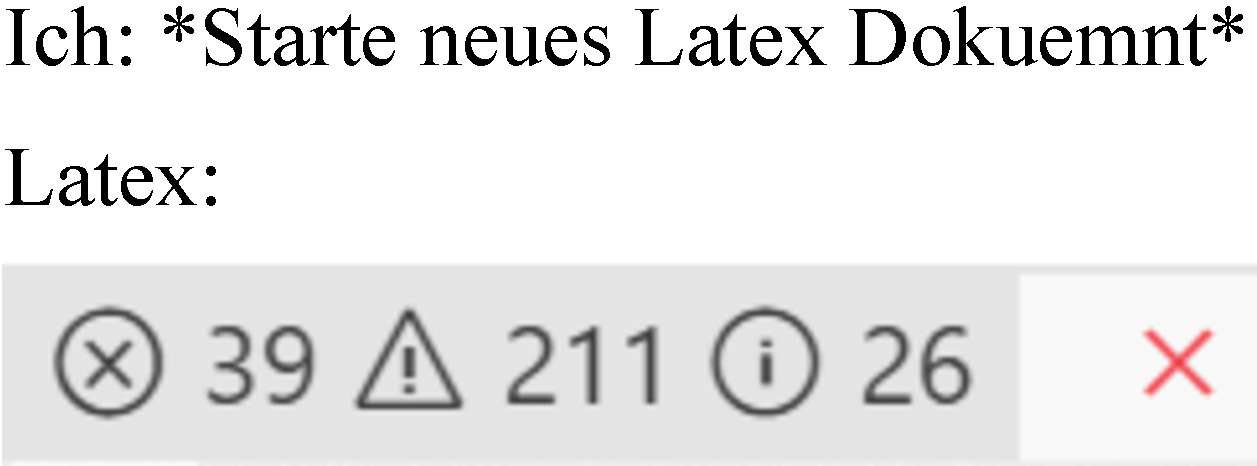
\includegraphics[width=0.35\textwidth]{img/25/memes/latexErrors.pdf}
    \caption{Wieder ein Meme}
\end{figure}

\newpage

\onecolumn
\begin{table}[h!]
    \vspace{-0.73cm}
    \centering
    \begin{tabular}{l|l|l|l||l}
    \toprule
    \textbf{Spannung [V/Div]} & \textbf{$\Delta V_{\text{Cursor}}$ [V]} & \textbf{$\Delta V_{2\times \text{Cursor}}$ [V]} & \textbf{$\Delta V_{\text{sys}}$ [V]} & \textbf{$\Delta V_{\text{gesamt}}$ [V]} \\
    \midrule
    \(2,00\times 10^{-3}\) & \(5,00\times 10^{-6}\) & \(1,41\times 10^{-4}\) & -- & -- \\
    \(5,00\times 10^{-3}\) & \(1,25\times 10^{-5}\) & \(3,54\times 10^{-4}\) & -- & -- \\
    \(1,00\times 10^{-2}\) & \(2,50\times 10^{-5}\) & \(7,07\times 10^{-4}\) & \(3,00\times 10^{-4}\) & \(7,68\times 10^{-4}\) \\
    \(2,00\times 10^{-2}\) & \(5,00\times 10^{-5}\) & \(1,41\times 10^{-3}\) & \(6,00\times 10^{-4}\) & \(1,54\times 10^{-3}\) \\
    \(5,00\times 10^{-2}\) & \(1,25\times 10^{-4}\) & \(3,54\times 10^{-3}\) & \(1,50\times 10^{-3}\) & \(3,84\times 10^{-3}\) \\
    \(1,00\times 10^{-1}\) & \(2,50\times 10^{-4}\) & \(7,07\times 10^{-3}\) & \(3,00\times 10^{-3}\) & \(7,68\times 10^{-3}\) \\
    \(2,00\times 10^{-1}\) & \(5,00\times 10^{-4}\) & \(1,41\times 10^{-2}\) & \(6,00\times 10^{-3}\) & \(1,54\times 10^{-2}\) \\
    \(5,00\times 10^{-1}\) & \(1,25\times 10^{-3}\) & \(3,54\times 10^{-2}\) & \(1,50\times 10^{-2}\) & \(3,84\times 10^{-2}\) \\
    \(1,00\) & \(2,50\times 10^{-3}\) & \(7,07\times 10^{-2}\) & \(3,00\times 10^{-2}\) & \(7,68\times 10^{-2}\) \\
    \(2,00\) & \(5,00\times 10^{-3}\) & \(1,41\times 10^{-1}\) & \(6,00\times 10^{-2}\) & \(1,54\times 10^{-1}\) \\
    \(5,00\) & \(1,25\times 10^{-2}\) & \(3,54\times 10^{-1}\) & \(1,50\times 10^{-1}\) & \(3,84\times 10^{-1}\) \\
    \midrule
    \midrule
    \textbf{Zeit [t/Div]} & \textbf{$\Delta_{\text{Cursor}}$ [s]} & \textbf{$\Delta t_{2\times \text{Cursor}}$ [s]} & \textbf{$\Delta t_{\text{sys}}$ [s]} & \textbf{$\Delta t_{\text{gesamt}}$ [s]} \\
    \midrule
\(5~\text{ns}\) & \(1,00\times 10^{-11}\) & \(3,16\times 10^{-10}\) & \(2,50\times 10^{-13}\) & \(3,16\times 10^{-10}\) \\
    \(10~\text{ns}\) & \(2,00\times 10^{-11}\) & \(6,32\times 10^{-10}\) & \(5,00\times 10^{-13}\) & \(6,32\times 10^{-10}\) \\
    \(20~\text{ns}\) & \(4,00\times 10^{-11}\) & \(1,26\times 10^{-9}\) & \(1,00\times 10^{-12}\) & \(1,26\times 10^{-9}\) \\
    \(50~\text{ns}\) & \(1,00\times 10^{-10}\) & \(3,16\times 10^{-9}\) & \(2,50\times 10^{-12}\) & \(3,16\times 10^{-9}\) \\
    \(100~\text{ns}\) & \(2,00\times 10^{-10}\) & \(6,32\times 10^{-9}\) & \(5,00\times 10^{-12}\) & \(6,32\times 10^{-9}\) \\
    \(200~\text{ns}\) & \(4,00\times 10^{-10}\) & \(1,26\times 10^{-8}\) & \(1,00\times 10^{-11}\) & \(1,26\times 10^{-8}\) \\
    \(500~\text{ns}\) & \(1,00\times 10^{-9}\) & \(3,16\times 10^{-8}\) & \(2,50\times 10^{-11}\) & \(3,16\times 10^{-8}\) \\
    \(1~\mu\text{s}\) & \(2,00\times 10^{-9}\) & \(6,32\times 10^{-8}\) & \(5,00\times 10^{-11}\) & \(6,32\times 10^{-8}\) \\
    \(2~\mu\text{s}\) & \(4,00\times 10^{-9}\) & \(1,26\times 10^{-7}\) & \(1,00\times 10^{-10}\) & \(1,26\times 10^{-7}\) \\
    \(5~\mu\text{s}\) & \(1,00\times 10^{-8}\) & \(3,16\times 10^{-7}\) & \(2,50\times 10^{-10}\) & \(3,16\times 10^{-7}\) \\
    \(10~\mu\text{s}\) & \(2,00\times 10^{-8}\) & \(6,32\times 10^{-7}\) & \(5,00\times 10^{-10}\) & \(6,32\times 10^{-7}\) \\
    \(20~\mu\text{s}\) & \(4,00\times 10^{-8}\) & \(1,26\times 10^{-6}\) & \(1,00\times 10^{-9}\) & \(1,26\times 10^{-6}\) \\
    \(50~\mu\text{s}\) & \(1,00\times 10^{-7}\) & \(3,16\times 10^{-6}\) & \(2,50\times 10^{-9}\) & \(3,16\times 10^{-6}\) \\
    \(100~\mu\text{s}\) & \(2,00\times 10^{-7}\) & \(6,32\times 10^{-6}\) & \(5,00\times 10^{-9}\) & \(6,32\times 10^{-6}\) \\
    \(200~\mu\text{s}\) & \(4,00\times 10^{-7}\) & \(1,26\times 10^{-5}\) & \(1,00\times 10^{-8}\) & \(1,26\times 10^{-5}\) \\
    \(500~\mu\text{s}\) & \(1,00\times 10^{-6}\) & \(3,16\times 10^{-5}\) & \(2,50\times 10^{-8}\) & \(3,16\times 10^{-5}\) \\
    \(1~\text{ms}\) & \(2,00\times 10^{-6}\) & \(6,32\times 10^{-5}\) & \(5,00\times 10^{-8}\) & \(6,32\times 10^{-5}\) \\
    \(2~\text{ms}\) & \(4,00\times 10^{-6}\) & \(1,26\times 10^{-4}\) & \(1,00\times 10^{-7}\) & \(1,26\times 10^{-4}\) \\
    \(5~\text{ms}\) & \(1,00\times 10^{-5}\) & \(3,16\times 10^{-4}\) & \(2,50\times 10^{-7}\) & \(3,16\times 10^{-4}\) \\
    \(10~\text{ms}\) & \(2,00\times 10^{-5}\) & \(6,32\times 10^{-4}\) & \(5,00\times 10^{-7}\) & \(6,32\times 10^{-4}\) \\
    \(20~\text{ms}\) & \(4,00\times 10^{-5}\) & \(1,26\times 10^{-3}\) & \(1,00\times 10^{-6}\) & \(1,26\times 10^{-3}\) \\
    \(50~\text{ms}\) & \(1,00\times 10^{-4}\) & \(3,16\times 10^{-3}\) & \(2,50\times 10^{-6}\) & \(3,16\times 10^{-3}\) \\
    \(100~\text{ms}\) & \(2,00\times 10^{-4}\) & \(6,32\times 10^{-3}\) & \(5,00\times 10^{-6}\) & \(6,32\times 10^{-3}\) \\
    \(200~\text{ms}\) & \(4,00\times 10^{-4}\) & \(1,26\times 10^{-2}\) & \(1,00\times 10^{-5}\) & \(1,26\times 10^{-2}\) \\
    \(500~\text{ms}\) & \(1,00\times 10^{-3}\) & \(3,16\times 10^{-2}\) & \(2,50\times 10^{-5}\) & \(3,16\times 10^{-2}\) \\
    \(1~\text{s}\) & \(2,00\times 10^{-3}\) & \(6,32\times 10^{-2}\) & \(5,00\times 10^{-5}\) & \(6,32\times 10^{-2}\) \\
    \(2~\text{s}\) & \(4,00\times 10^{-3}\) & \(1,26\times 10^{-1}\) & \(1,00\times 10^{-4}\) & \(1,26\times 10^{-1}\) \\
    \(5~\text{s}\) & \(1,00\times 10^{-2}\) & \(3,16\times 10^{-1}\) & \(2,50\times 10^{-4}\) & \(3,16\times 10^{-1}\) \\
    \(10~\text{s}\) & \(2,00\times 10^{-2}\) & \(6,32\times 10^{-1}\) & \(5,00\times 10^{-4}\) & \(6,32\times 10^{-1}\) \\
    \(20~\text{s}\) & \(4,00\times 10^{-2}\) & \(1,26\times 10^{0}\) & \(1,00\times 10^{-3}\) & \(1,26\times 10^{0}\) \\
    \(50~\text{s}\) & \(1,00\times 10^{-1}\) & \(3,16\times 10^{0}\) & \(2,50\times 10^{-3}\) & \(3,16\times 10^{0}\) \\
    \bottomrule
    \end{tabular}
    \caption{Spannungs- und Zeitauflösung, systematische Fehler und Gesamtfehler des Oszilloskops. Berücksichtigung von Ablese- und Systematischenfehlern.}
    \label{tab:all_fehler}
\end{table}
\twocolumn





